% CHAPITRE 3
\chapter{Bilan de C de la tourbière de La Guette}

\minitoc

\newpage

\section{Introduction}

Afin de pouvoir interpoler les mesures de respiration mensuelles, il est nécessaire de les relier à des variables environnementales nous l'avons vu.
Un des facteurs de contrôle des flux est la température qui régule les processus chimiques et biologiques.
La température à \SI{-5}{\cm} est la plus souvent utilisée \cite{ballantyne2014}, même si d'autres comme la température de l'air ou encore la température du sol à \SI{-10}{\cm} peuvent également l'être \cite{bortoluzzi2006,kim1992}.
Cette profondeur, \SI{-5}{\cm}, est régulièrement utilisée car c'est dans la tourbe, proche de la surface qu'est produit la majorité du \coo.
\textbf{production CO2 ? profils ?}
C'est également à des profondeurs relativement faibles que se situent la majorité des racines \plop qui peuvent contribuer à la respiration du sol \textbf{(de l'écosystème?)} pour 35 à \SI{60}{\percent} \cite{silvola1996,crow2005}.

Objectif : bilan de C


\section{Procédure expérimentale et analytique}

\subsection{Méthodes de mesure}

\subsubsection{Mesures de flux de gaz}
La mesure des flux de \coo et de \chh ont été effectué en utilisant la méthode décrite dans la partie~\ref{sec:clsd_chbr_method}.
En XmoisX YannéeY, 20 placettes ont été installées\footnote{je remercie ici Sébastien Gogo pour avoir installé ces placettes sur le terrain avant même mon arrivée.} selon un échantillonnage aléatoire stratifié:
La surface de la tourbière a été divisée selon une grille de 20 mailles et un point choisi aléatoirement dans chaque maille localise chaque placette.
Cette méthode permet de conserver un échantillonnage aléatoire tout en étant assuré d'avoir une représentativité homogène du site. 
Les placettes, délimitées par des piquets, occupaient une surface de \SI{4}{\square\metre} (2$\times$\SI{2}{\metre}), à l'intérieur de laquelle ont été installé de façon permanente un piézomètre et une embase permettant la mesure des flux de gaz.
Usuellement les placettes sont séparées en groupes micro-topographique. ce qui à l'avantage de permettre une distinction des capacités sources/puits relativement fine mais qui à généralement l'inconvénient du placement proche des embases les unes des autres.
Elles peuvent également être séparées en zone dans la tourbière, haut-marais par rapport à bas-marais, ou réhabilité par rapport à non-réhabilité.
Afin de gagner en représentativité spatiale, la taille du site le permettant, il a donc été décidé de positionner des placettes sur l'ensemble du site.
De plus, du fait de l'omniprésence de végétation vasculaire, et de la taille des chambres par rapport à la micro-topographie une telle approche était difficile à mettre en oeuvre.

Les mesures de \coo ont été effectué de mars 2013 à février 2015, avec une fréquence quasiment mensuelle (20 campagnes, pour 24 mois de mesure).

Les mesures de \chh ont été effectuées avec une fréquence moindre principalement liée au difficulté de mise en oeuvre de l'instrument SPIRIT (lourd, difficilement transportable dans un milieu tourbeux).

\subsubsection{Les facteurs contrôlants}

Les mesures manuelle effectuées sont la mesure de la pression atmosphérique, du PAR, des températures du sol à différentes profondeur, de la végétation.
Des prélèvements d'eau ont également été effectué chaque mois, une mesure du pH et de la conductivité dans cette eau a été réalisée sur le terrain après les mesures de flux puis les échantillons ont été congelés avant d'être analysé en terme de concentration de carbone dissous.
Ces mesures nécessitant d'accéder aux placettes régulièrement, des planches de bois ont été utilisées comme pontons mobiles, la dispersion des placettes sur le site rendant impossible une installation plus permanente.

Les mesures automatiquement acquise via une station météo campbell sont la température de l'air, température de la tourbe à X, X et X profondeur, vitesse et direction du vent, humidité relative de l'air, irradiation solaire, pression atmosphérique.

\subsection{Modélisation du bilan de C}
%principe général
\subsubsection{Démarche générale}
%Le bilan de C considéré ici est constitué de 3 éléments majeurs, le \coo, le \chh et de COD.
%Le \coo et de \chh sont regroupés dans ce qui est appelé bilan de GES.
%
%Afin d'établir un modèle empirique permettant de relier les émission de GES du site à des facteurs contrôlant à l'échelle de l'écosystème, les données acquises mensuellement ont été moyennées par campagne de mesure.
Afin de calculer le bilan de carbone du site il est nécessaire d'établir des modèles empiriques des flux afin de pourvoir interpoler les données acquises mensuellement sur l'ensemble des deux années de mesure.
Pour établir ces modèles empiriques les données acquises ont été moyennées par campagne de mesure.
Ceci permettant, dans un premier temps, de s'affranchir de la variabilité spatiale des flux pour se concentrer sur la variabilité temporelle.
Les relations entre flux et facteurs contrôlant ont ensuite été étudiées deux à deux.

Les flux de \coo ont été modélisé en partant de l'équation ENE = PPB - RE, et le bilan a été établi en estimant de façon séparée la PPB et la RE.
Cette séparation permettant de distinguer si une variation du bilan est liée à l'un ou l'autre des flux ou bien aux deux.
Les flux en phase gazeuse ont été modélisé en partant d'équation usuellement utilisées et dans lesquelles la température est le facteur contrôlant majeur.
Puis les résidus\footnote{Valeurs moyennes - Valeurs moyennes estimées} de ces modèles de base ont ensuite été étudiés en fonction des facteurs de contrôle restant.
Dans le cas ou une tendance est visible, le facteur est intégré.
Les modèles ont été comparés avec différents indicateurs, principalement Le R2, la NRMSE et l'AIC.
Le R$^{2}$ est utilisé comme indicateur de la proportion de la variabilité des données expliqué par le modèle, sa valeur est comprise entre 0 et 1.
La RMSE et sa normalisation par la moyenne NRMSE sont utilisés comme indicateur de l'écart entre les données mesurées et les données modélisées.
L'AIC (Akaile...) permet de déterminer si l'amélioration d'un modèle suite à l'ajout d'un paramètre est suffisamment intéressante pour que ce modèle plus complexe soit utilisé.

La température a été choisie comme base de départ à la construction des modèles de RE et PPBsat, à la fois car c'est le facteur de contrôle le plus souvent invoqué et à la fois car les corrélations avec les flux étaient les plus forte.
Idéalement la température utilisée pour estimer la photosynthèse serait celle de l'air et celle pour estimer la respiration serait celle du sol à faible profondeur, typiquement \SI{-5}{\centi\metre}.
En effet ce sont celles qui font le plus sens, la photosynthèse prenant place dans l'air et la majorité de la respiration se faisant dans les premiers centimètres du sol.
Ce sont également celles qui sont le plus utilisées dans la littérature.
Cependant les température de l'air mesurée manuellement au niveau de chaque embase lors des différentes campagnes de mesures, sont sujette à caution 
En effet elles sont quasiment certainement sur-estimées et donc biaisées.
La source de ce biais est la difficulté de maintenir à l'ombre de thermomètre utilisé lors des campagnes.
La température affichée par ce dernier ayant tendance à monter drastiquement quand exposé au soleil.
A l'inverse les températures mesurées dans le sol sont plus fiable (\textbf{pourquoi ?}).
L'utilisation de ces deux températures conjointement pour l'estimation d'un bilan risquant donc de le déséquilibrer il a été décider d'utiliser la température à \SI{-5}{\centi\metre} à la fois pour la RE mais aussi pour la PPB, ceci afin de pouvoir conserver une calibration issue de données locale et néanmoins robuste.
L'autre solution aurait été d'utiliser les données de température de la station pour la calibration.

Après cette phase de calibration, les facteurs de contrôle utilisés dans les modèles ont été interpolés au pas de mesure de la station météo présente sur le site, c'est à dire à l'heure.
L'interpolation étant soit une simple interpolation linéaire entre les données mensuelles, soit une relation avec les facteurs acquis par la station météorologique.
À l'aide de ces interpolations et des équations les flux ont ensuite été recalculés sur les 2 années de mesure.

Enfin ces modèles ont été évalués sur des données issues d'une autre expérimentation.On ne parle pas ici de validation car les données utilisées bien qu'indépendante du jeu de données utilisé pour la calibration n'ont pas été acquise suivant un protocole identique, notamment au niveau de la répartition des embases sur le site.


\subsubsection{La Production Primaire Brute}




%%%%%%%%%%%%%%%%%%%%% PPB 

L'estimation de la PPB se fait en deux temps.
Le premier consiste à estimer le potentiel maximum de photosynthèse à un instant donné dans des conditions de lumière saturante.
Ce potentiel peut varier avec les conditions environnementales.
Il est estimé en partant de l'équation de \cite{june2004}

Modélisation de la production primaire brute à lumière saturante.
L'utilisation de l'équation de June se justifie par ?

\begin{equation}\label{eq:juneTair}
PPBsat = a * exp(\frac{Tair - b}{c}^2)
\end{equation}

\begin{figure}
\centering
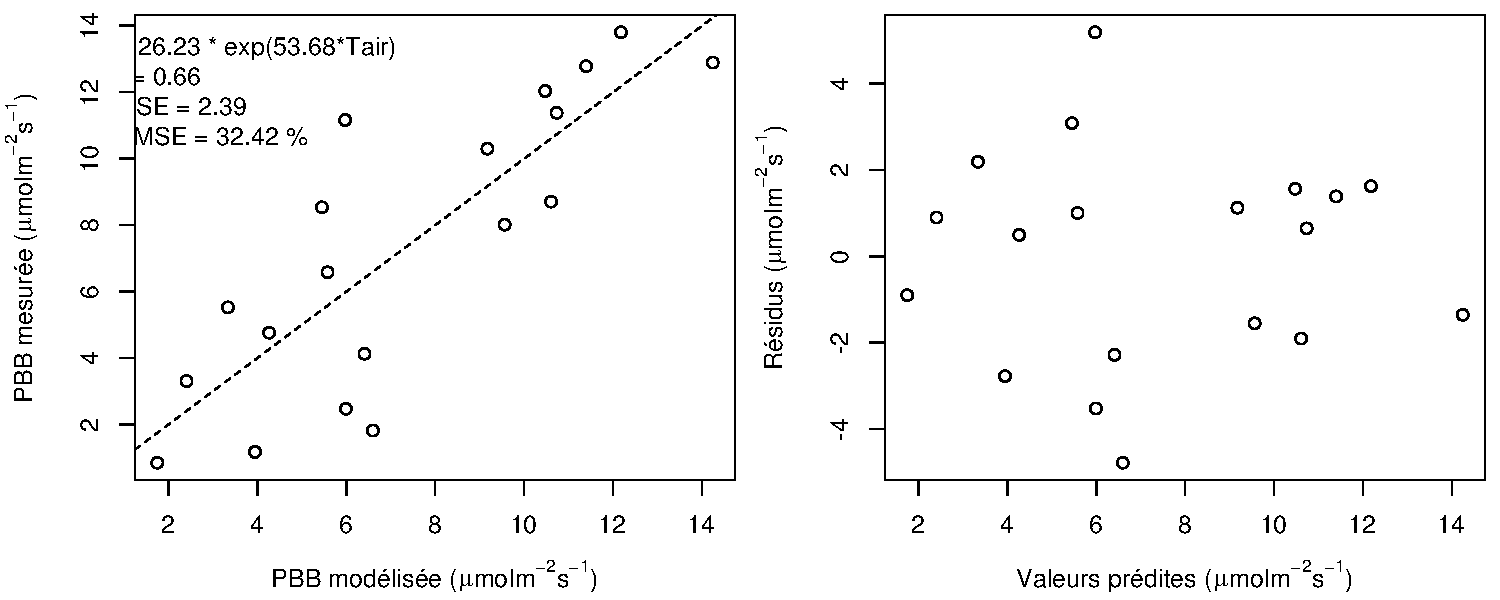
\includegraphics[width=\textwidth]{chap3/GPPsat_Tair_mdl_mesmod}
\caption{PPBsat modèles Tair utilisant l'équation~\ref{eq:juneTair}}
\label{fig:PPBsat_Tair_mdl}
\end{figure}

\begin{figure}
\centering
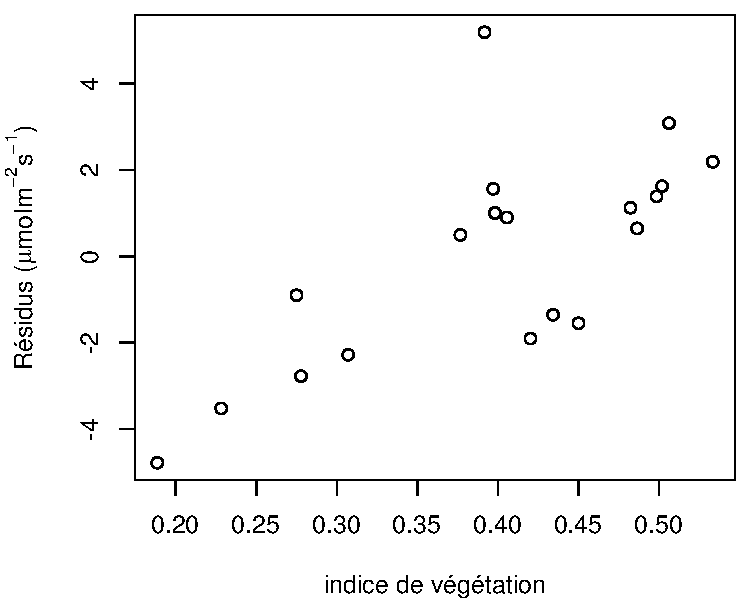
\includegraphics[width=.5\textwidth]{chap3/GPPsat_Tair_mdl_res}
\caption{Résidus de l'équation~\ref{eq:juneTair} en fonction de l'indice de végétation}
\label{fig:PPBsat_Tair_res}
\end{figure}

L'utilisation de l'équation de June seule, avec la température de l'air comme variable explicative de la PPBsat, permet d'expliquer 65 \% des variations observées (Figure~\ref{fig:PPB_Tair_mdl}).

RMSE ?

Les résidus de ce modèle se répartissent de façon relativement homogène et sans tendance.


\begin{figure}
\centering
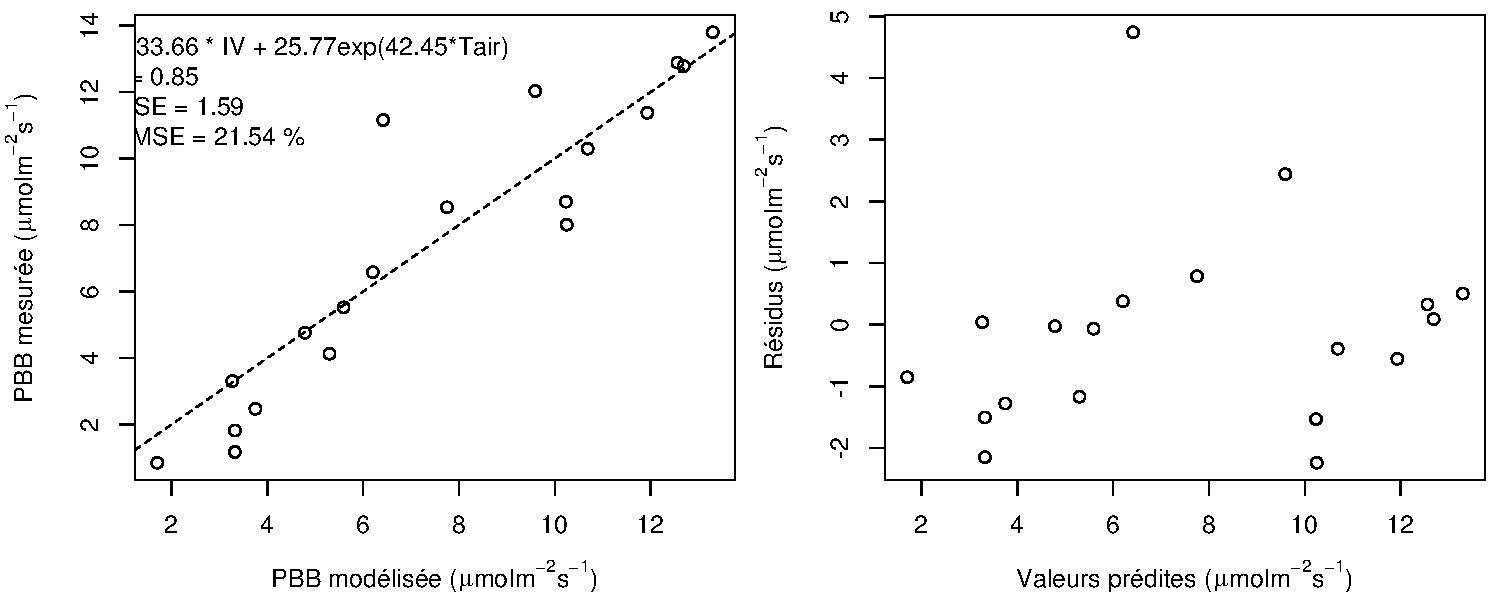
\includegraphics[width=\textwidth]{chap3/GPPsat_TairIV_mdl_mesmod}
\caption{PPBsat modèles Tair utilisant l'équation~\ref{eq:juneTairIV}}
\label{fig:PPBsat_TaIV_mdl}
\end{figure}

Lorsque qu'ils sont corrélés avec d'autres facteurs contrôlant important, le niveau de la nappe, la teneur en eau du sol, et un indice de végétation ils ne montrent de tendance qu'avec ce dernier (Figure~\ref{fig:PPBsat_Tair_res}).
Il semble y avoir une relation linéaire entre les résidus de l'équation et l'indice de végétation.
Le modèle est donc transformé en 

\begin{equation}\label{eq:juneTairIV}
PPBsat = (a * IV + b) * exp(\frac{T - b}{c}^2)
\end{equation}

Cette nouvelle équation permet d'expliquer une part plus importante des variations de PPBsat (R$^{2}$ = 0,86) et augmente la proximité entre les données mesurées et les données modélisées (La RMSE diminue) (Figure~\ref{fig:PPB_TairIV_mdl}).
Les résidus de cette équation sont, à l'exception d'un point, répartis de façon homogène autour de 0, sans tendance particulière.

À partir de ce potentiel la PPB est estimée en prenant en compte la luminosité.
Deux équations ont été testées :

\begin{equation} \label{eq:PPB_bubier}
PPB = \frac{PPBsat * a * PAR}{PPBsat + a * PAR}
\end{equation}

\begin{equation} \label{eq:PPB_sig}
PPB = \frac{PPBsat * a * PAR}{\sqrt{PPBsat^2 + (a * PAR)^2}}
\end{equation}

L'équation~\ref{eq:PPB_bubier} a été proposée par \cite{bubier1998} et utilisée par \cite{bortoluzzi2006,worrall2009} et tandis que l'équation~\ref{eq:PPB_sig}, plus rarement utilisée a été introduite par \cite{smith1937} et utilisée par \cite{wohlfahrt2010,gorres2014}.


\begin{figure}
\centering
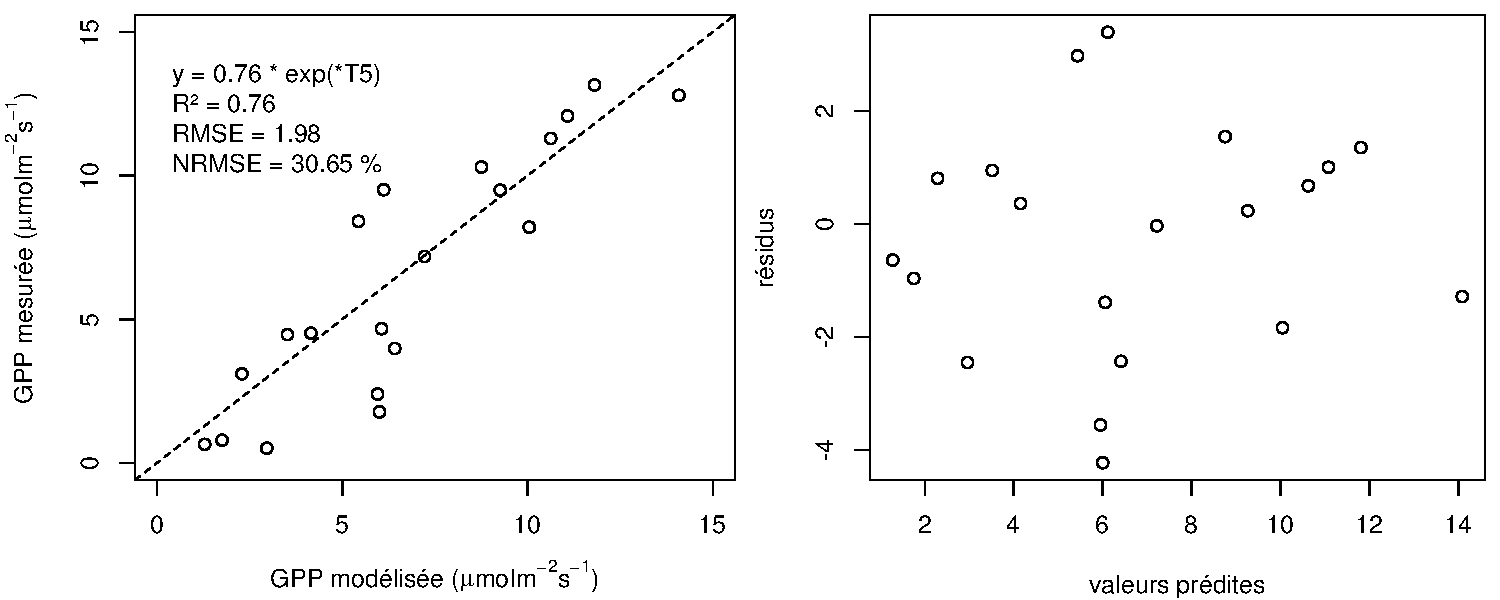
\includegraphics[width=\textwidth]{chap3/GPP_Tair_mdl_mesmod}
\caption{PPB modèles Tair}
\label{fig:PPB_Tair_mdl}
\end{figure}

\begin{figure}
\centering
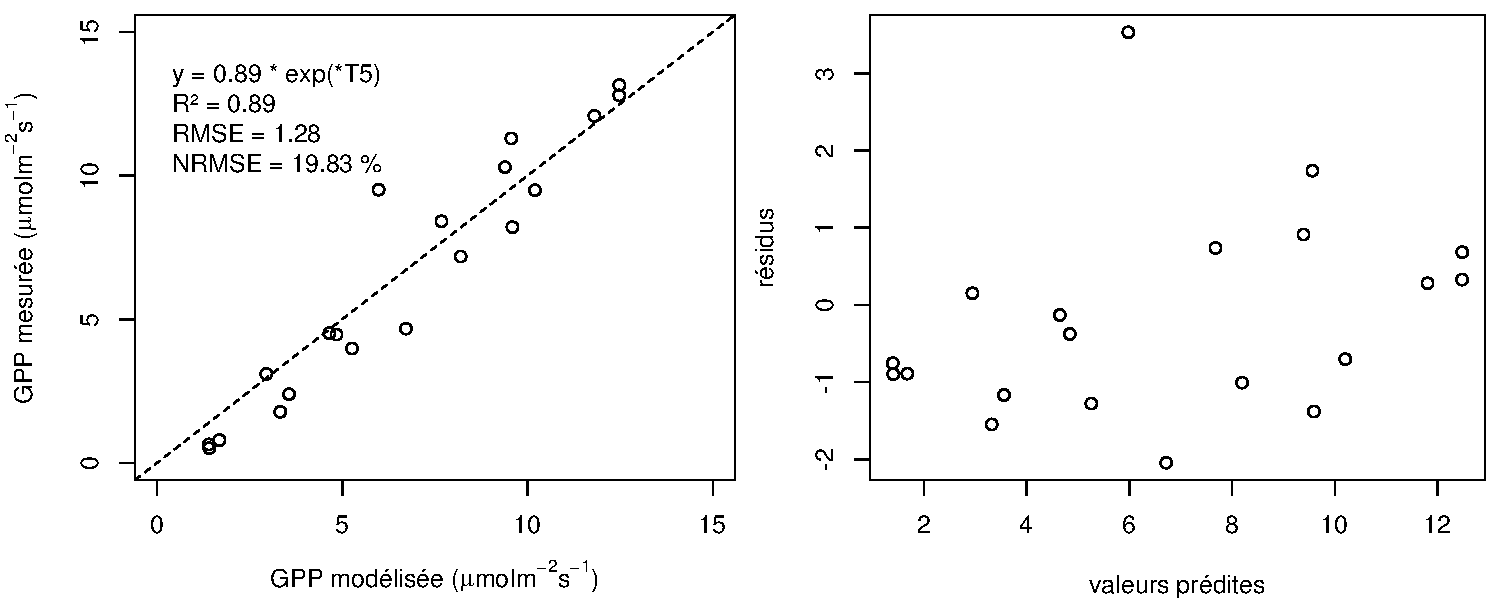
\includegraphics[width=\textwidth]{chap3/GPP_TairIV_mdl_mesmod}
\caption{PPB résidus modèle Tair}
\label{fig:PPB_TairIV_mdl}
\end{figure}

\subsubsection{La Respiration de l'Écosystème}

%%%%%%%%%%%%%%%%%%%%% RE

La RE est estimée directement à partir des données acquises moyennées en partant de la température connue pour contrôler une grande partie de ce flux.
Différents modèles ont été testés parmi les plus souvent utilisés (linéaire, exponentiel, arrhénius).


Les variations de la RE moyenne au cours du temps suivent les variations saisonnières de la température.

\begin{equation} \label{eq:RE_T5}
RE = a*exp(b*T5)
\end{equation}

La température de l'air utilisée dans un modèle exponentiel permet d'expliquer une grande partie, 90 \%, des variations de la respiration de l'écosystème (Figure~\ref{fig:ER_T5_mdl}).
Les résidus de cette équation semble répartis de façon non-biaisée, pas de tendance dans le nuage de point (Figure~\ref{fig:ER_T5_mdl}). 
Comme pour la GPPsat, la seule tendance qui semble se dégager lorsque que l'on corrèle ces résidus aux autres facteurs contrôlant, est une tendance linéaire avec l'indice de végétation (Figure~\ref{fig:ER_T5_res}).
Cependant l'ajout d'un paramètre avec un gain forcément limité ne semble pas utile/pertinent.

\begin{figure}
\centering
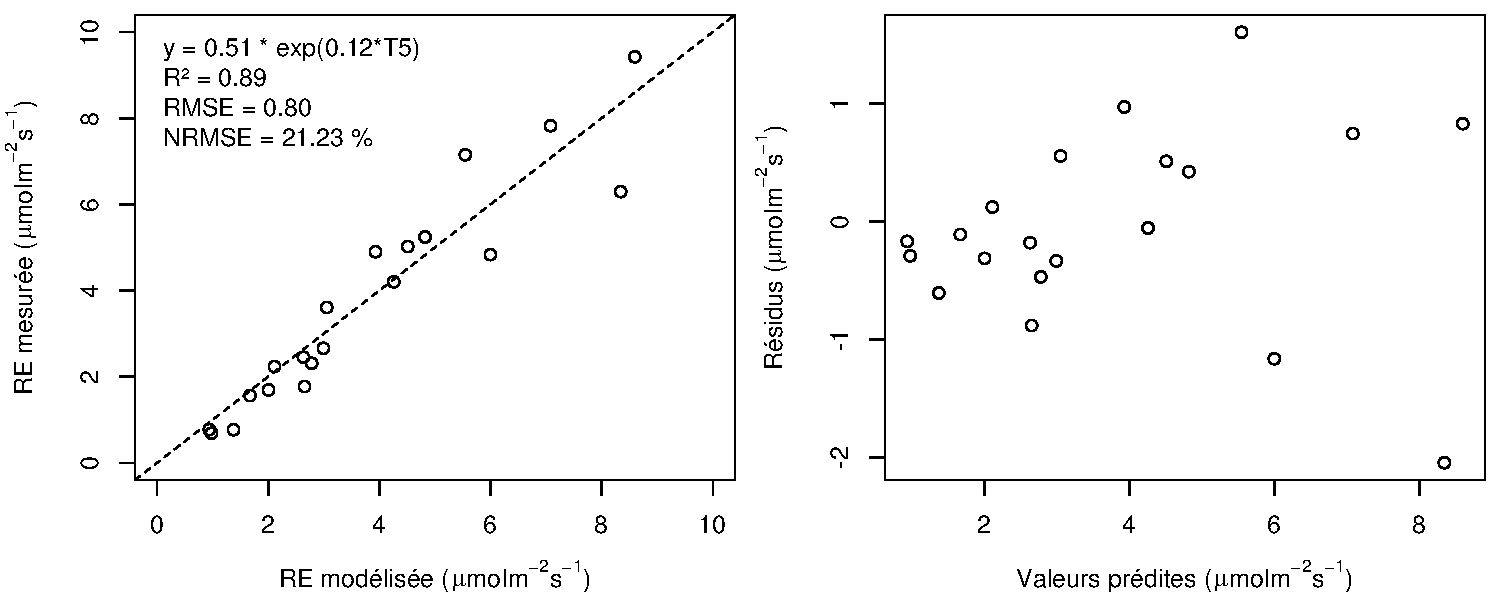
\includegraphics[width=\textwidth]{chap3/ER_T5_mdl_mesmod}
\caption{RE modèles avec T5}
\label{fig:ER_T5_mdl}
\end{figure}

\begin{figure}
\centering
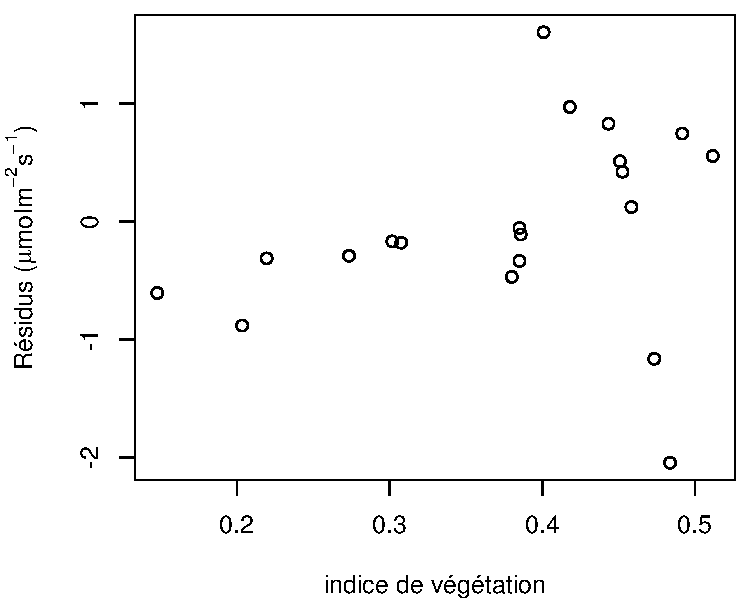
\includegraphics[width=.5\textwidth]{chap3/ER_T5_mdl_res}
\caption{RE, résidus du modèle avec T5}
\label{fig:ER_T5_res}
\end{figure}

%%%%%%%%%%%%%%%%%%%%% ENE

L'ENE est ensuite modélisé en utilisant l'équation suivante :

\begin{equation}
ENE = PBB-RE
\end{equation}

Le résultat de cette équation (Figure~\ref{fig:ENE_T5_mdl}), montre que ce modèle permet d'expliquer une grande partie des variations de l'ENE.
Les résidus de cette équation sont répartis de manière a peu près homogène.

\begin{figure}
\centering
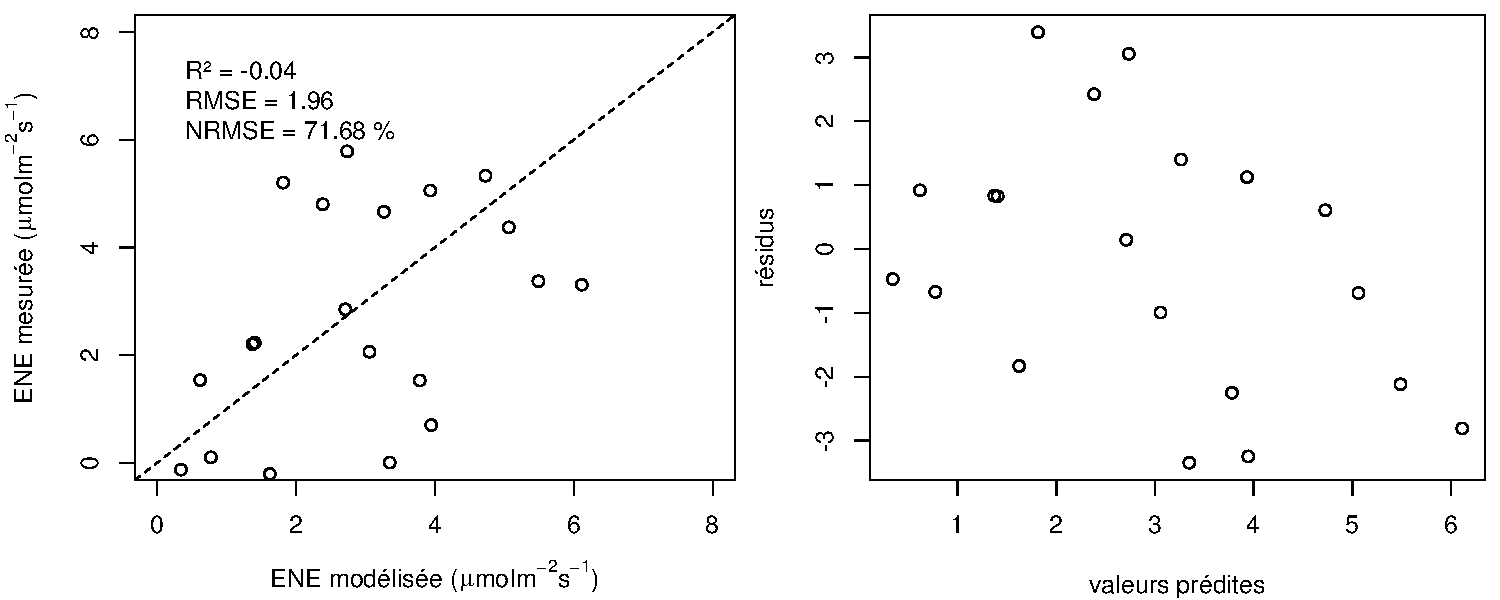
\includegraphics[width=\textwidth]{chap3/NEE_Tair-T5_mdl_mesmod}
\caption{ENE modèle T5 IV}
\label{fig:ENE_T5_mdl}
\end{figure}

\begin{figure}
\centering
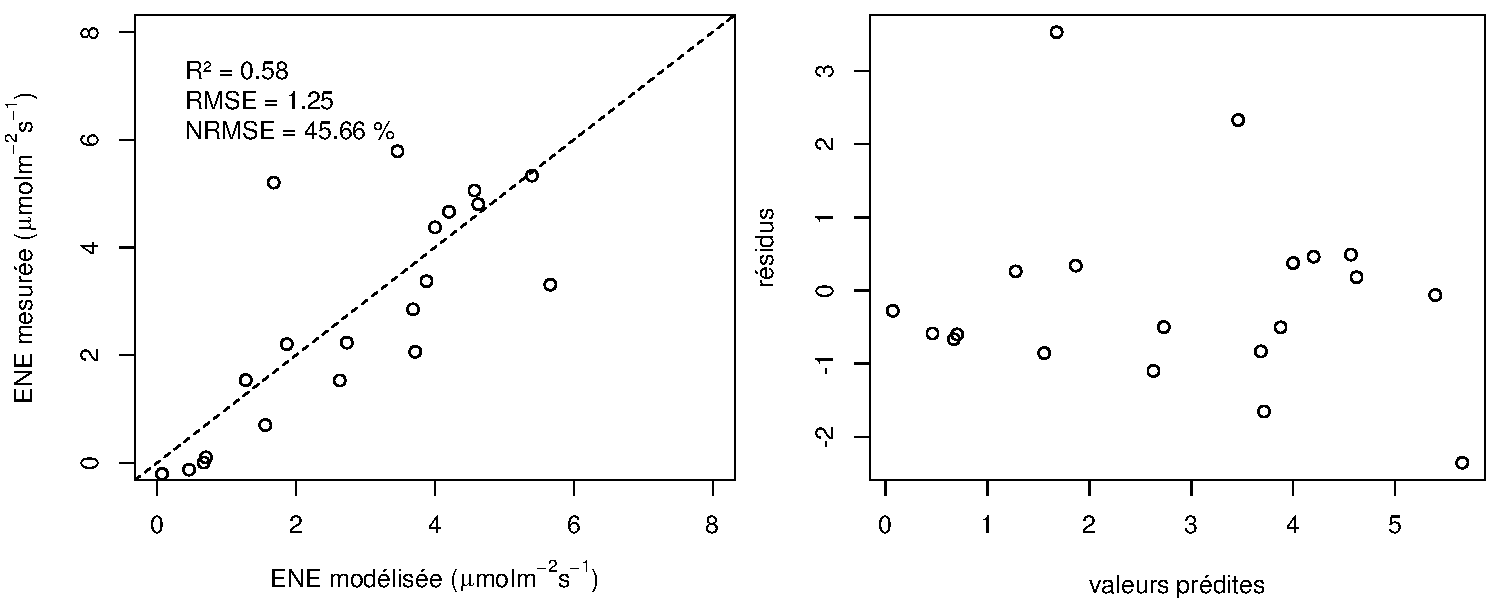
\includegraphics[width=\textwidth]{chap3/NEE_TairIVcov-T5_mdl_mesmod}
\caption{ENE modèle T5 IV}
\label{fig:ENE_T5IV_mdl}
\end{figure}

\subsubsection{Le flux de \chh}

\subsubsection{Le COD}

\section{Résultats}

\subsection{Évolution générale des facteurs contrôlants sur la tourbière de La Guette}

L'évolution du niveau de la nappe des 20 placettes, décrite dans la figure~\ref{fig:WTL_mean_evolution}, est marquée par un étiage d'une vingtaine de centimètres en moyenne en 2013 et l'absence d'un étiage net en 2014 avec un niveau de la nappe moyen ne descendant que rarement sous la barre des \SI{-10}{\cm}.
Ces observations sont cohérentes avec la figure~\ref{fig:WTL} représentant des données acquises à plus haute fréquence, et confirment la particularité de ces 2 années vis à vis des précédentes qui présentent des étiages bien plus fort.

\begin{figure}
\centering
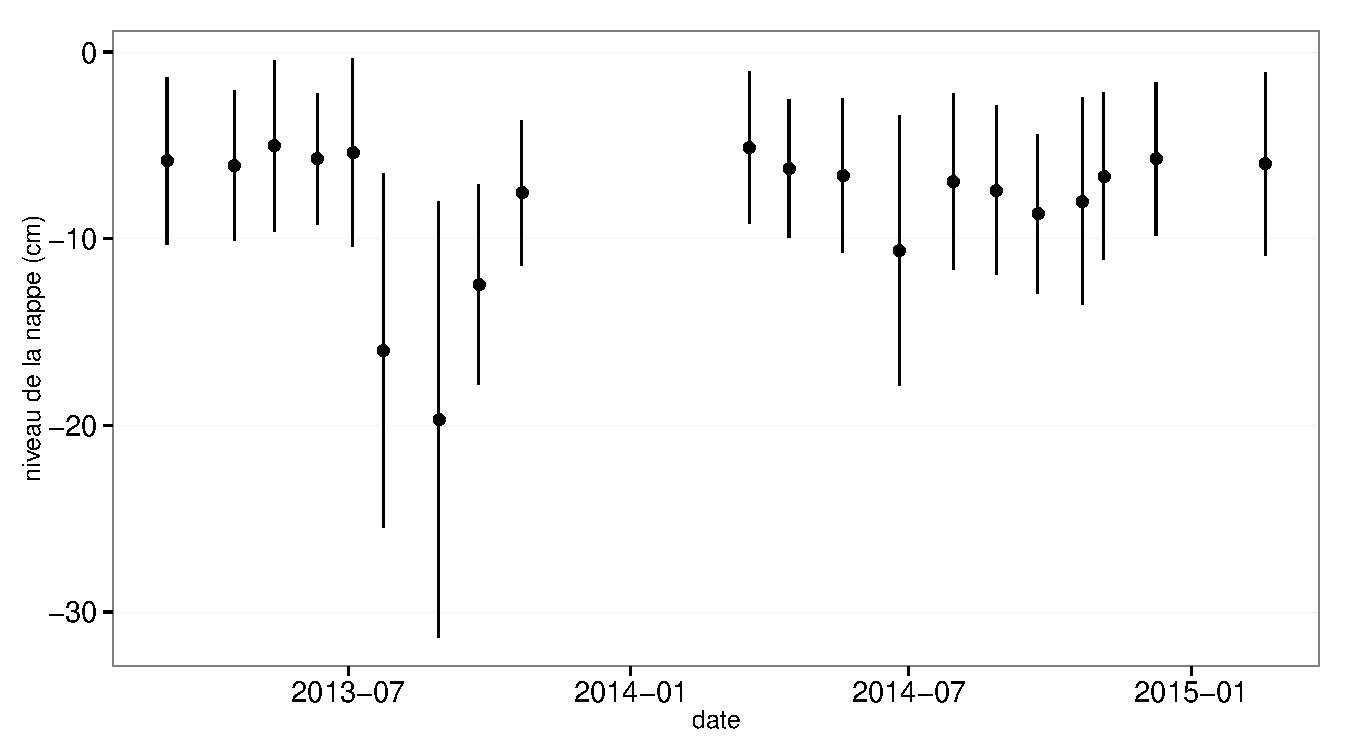
\includegraphics[width=\textwidth]{chap3/WTL_mean_evolution}
\caption{Évolution du niveau de la nappe moyen des 20 embases mesuré pendant la période de mesure (mars 2013 -- février 2015)}
\label{fig:WTL_mean_evolution}
\end{figure}

La température de l'air mesurée manuellement montre une variabilité saisonnière cohérente avec celle mesurées par la station météo. 
%bien que les valeurs semblent systématiquement supérieures.
La variabilité saisonnière de la température est également visible dans le sol avec cependant un amortissement et une diminution de la variabilité avec la profondeur (figure~\ref{fig:T_mean_evolution})
%chiffres ?


\begin{figure}
\centering
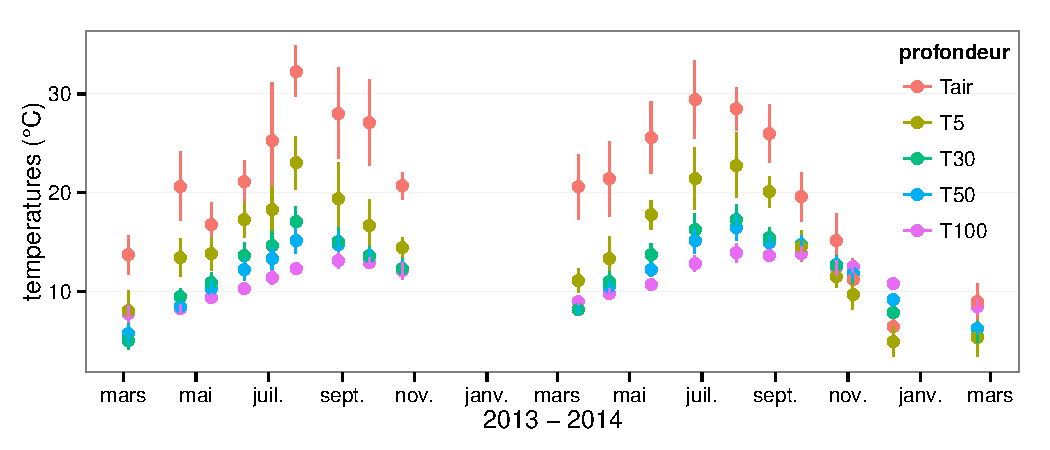
\includegraphics[width=\textwidth]{chap3/T_mean_evolution}
\caption{Évolution des températures de l'air (Tair) et du sol à \SIlist{-5;-30;-50;-100}{\centi\metre} (T5, T30, T50 et T100 respectivement) moyenne mesurée lors des campagnes de terrain de mars 2013 à février 2015}
\label{fig:T_mean_evolution}
\end{figure}

La conductivité moyenne mesurée sur le site varie entre \SIlist{35;55}{\usml} (figure~\ref{fig:cond_mean_evolution}).

\begin{figure}
\centering
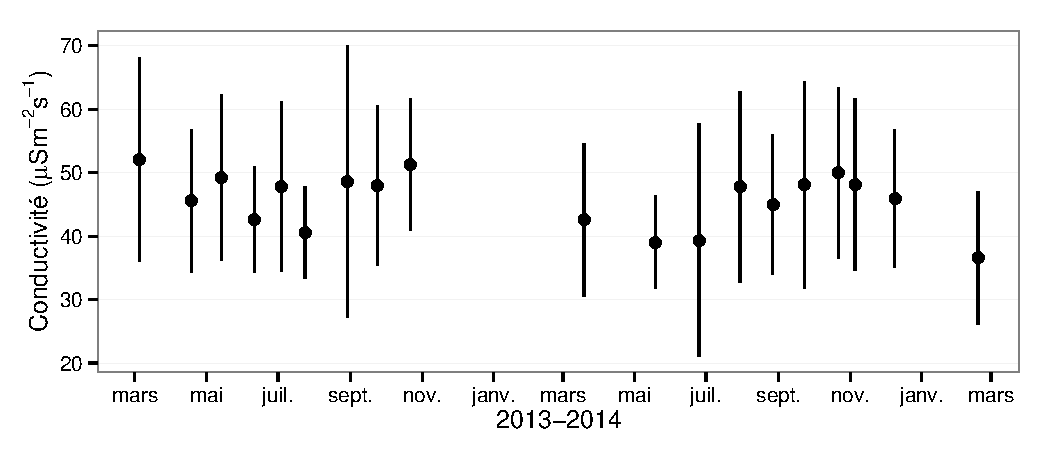
\includegraphics[width=\textwidth]{chap3/cond_mean_evolution}
\caption{Évolution de la conductivité pendant la période de mesure (mars 2013 -- février 2015)}
\label{fig:cond_mean_evolution}
\end{figure}

En moyenne le pH mesuré sur la tourbière de La Guette est compris entre 4 et 5 (figure~\ref{fig:pH_mean_evolution}).
Ces valeurs sont cohérentes avec la classification \textit{poor-fen} du site .

\begin{figure}
\centering
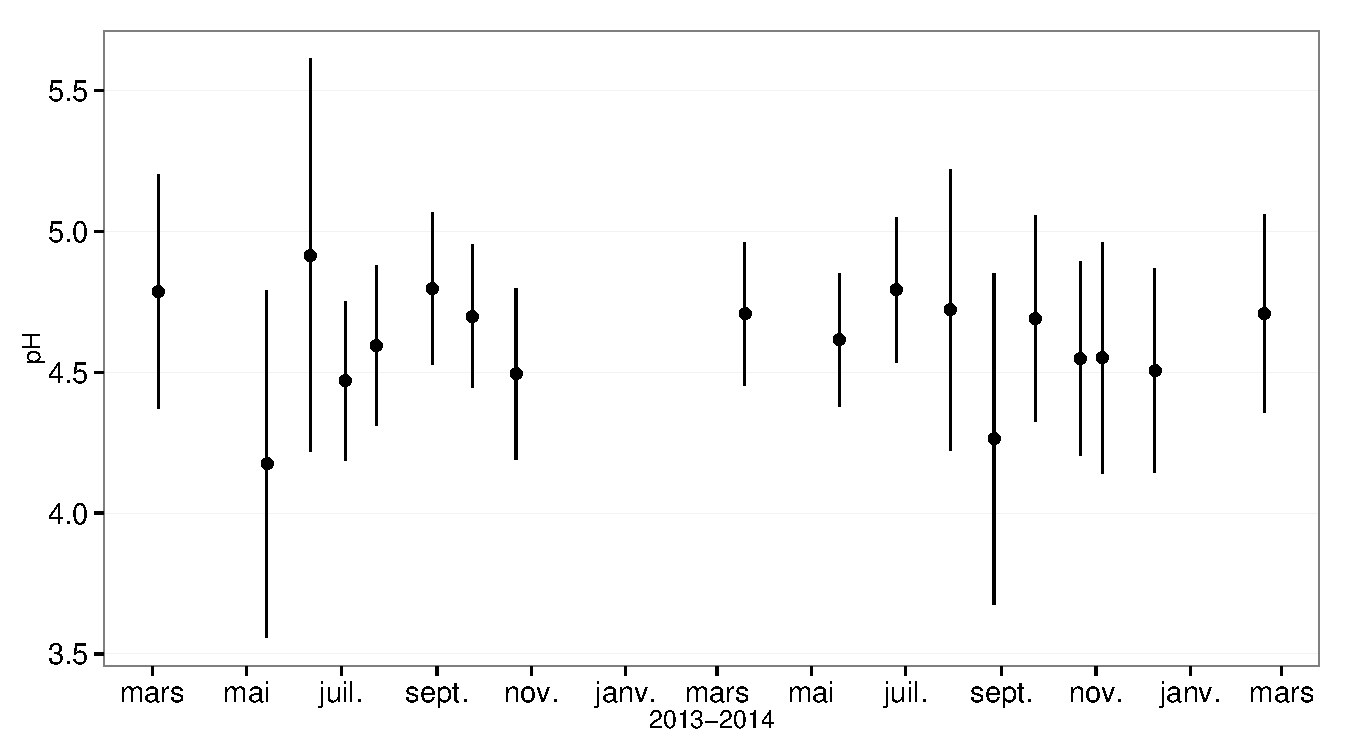
\includegraphics[width=\textwidth]{chap3/pH_mean_evolution}
\caption{Évolution du pH pendant la période de mesure (mars 2013 -- février 2015)}
\label{fig:pH_mean_evolution}
\end{figure}


\begin{figure}
\centering
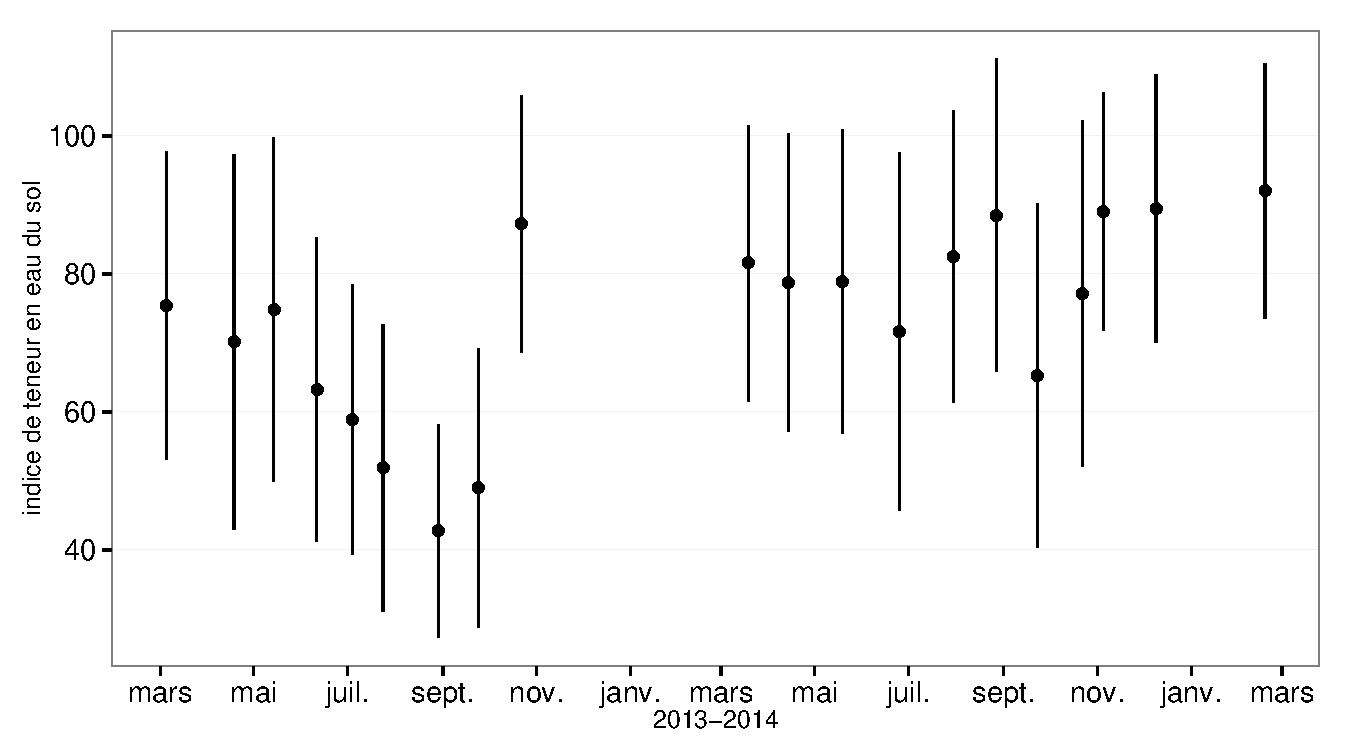
\includegraphics[width=\textwidth]{chap3/RH_mean_evolution}
\caption{Évolution de la teneur en eau du sol pendant la période de mesure (mars 2013 -- février 2015)}
\label{fig:RH_mean_evolution}
\end{figure}

\subsection{Évolution générale des flux de C sur la tourbière de La Guette}

\subsubsection{Le \coo}

\begin{figure}
	\centering
	\begin{subfigure}[t]{\textwidth}
		\centering
		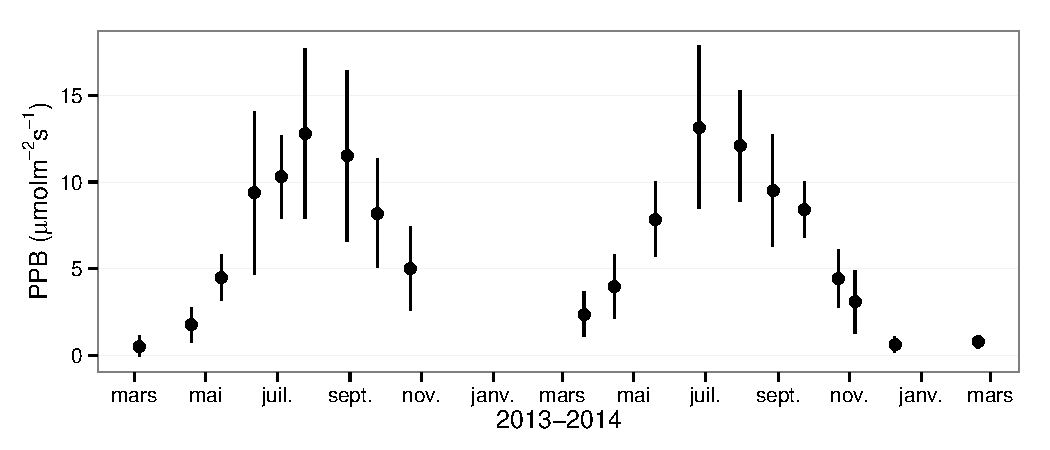
\includegraphics[width=\textwidth]{chap3/GPP_evolution_avg}
		\caption{Production primaire brute}
		\label{fig:GPP_evolution_avg}
	\end{subfigure}%
	
	\begin{subfigure}[t]{\textwidth}
		\centering
		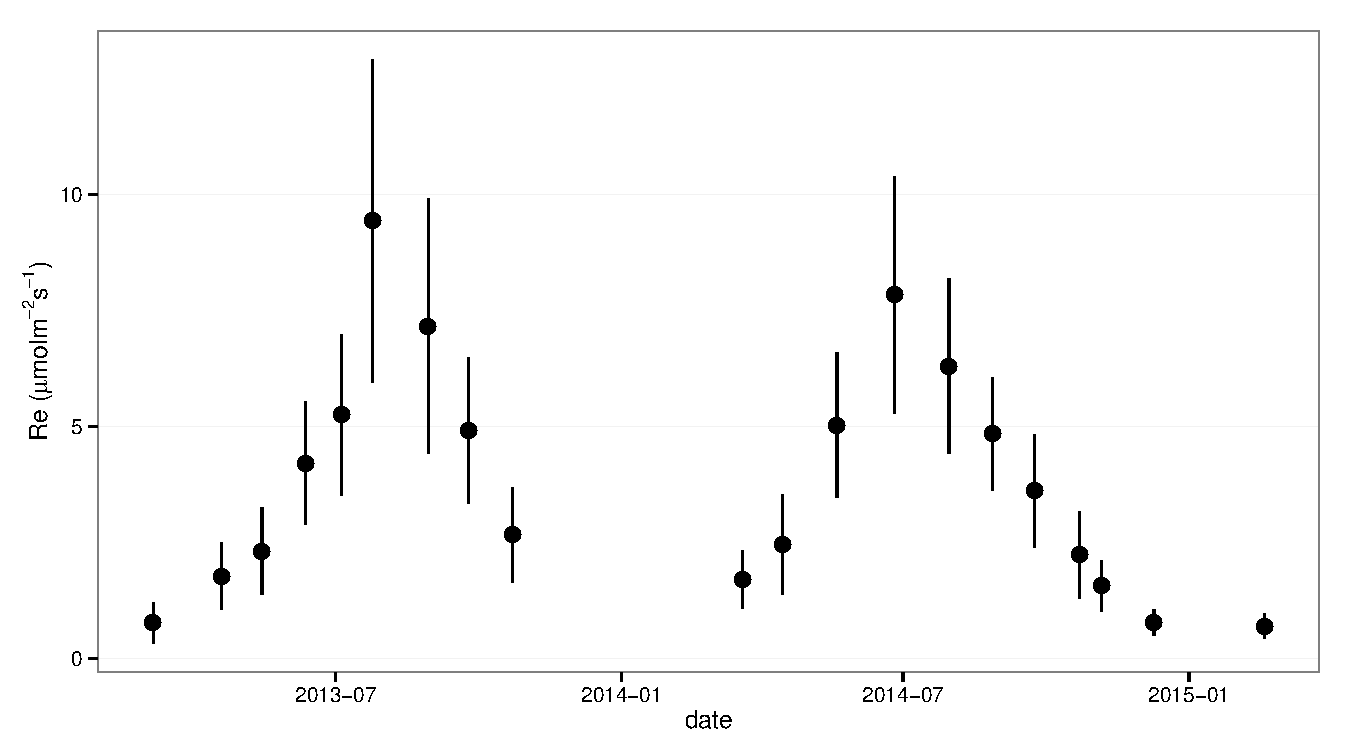
\includegraphics[width=\textwidth]{chap3/ER_evolution_avg}
		\caption{Respiration de l'écosystème}
		\label{fig:ER_evolution_avg}
	\end{subfigure}
	
	\begin{subfigure}[t]{\textwidth}
		\centering
		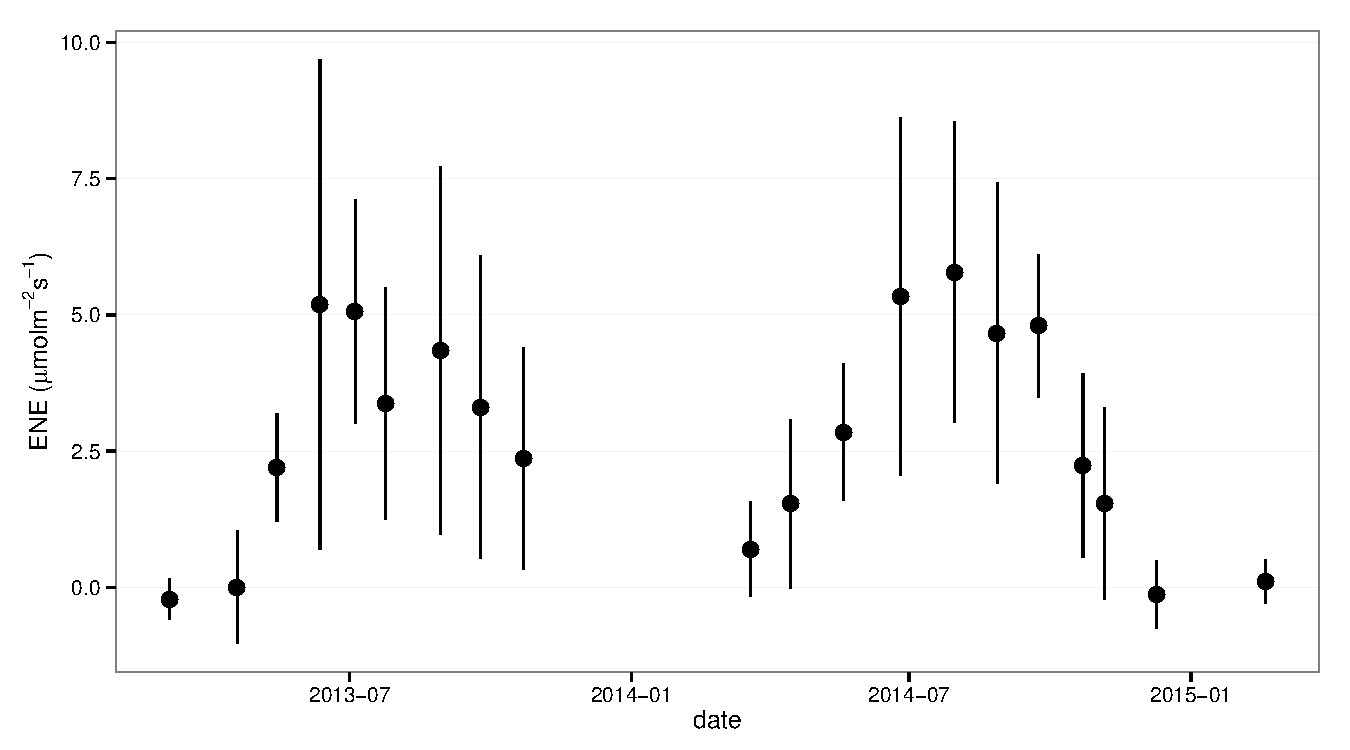
\includegraphics[width=\textwidth]{chap3/NEE_evolution_avg}
		\caption{Échange net de l'écosystème}
		\label{fig:NEE_evolution_avg}
	\end{subfigure}
\caption{Évolution du niveau de PPB, RE et ENE pendant la période de mesure. Moyenne des 20 embases de mars 2013 à février 2015.}
\label{fig:flux_evolution_avg}
\end{figure}

%\subsubsection{PBB}
L'ensemble des mesures de \coo s'étendent de mars 2013 à février 2015.
Cependant de novembre 2013 à février 2014 les mesures ont été interrompue suite à des pannes/casses matérielles.
Malgré cela les périodes les plus critiques, notamment la saison de végétation, ont pu être mesurées pour les 2 années, permettant d'avoir une vision correcte/globale de chacune d'elle.
À noter également que pour l'ensemble des flux, la déviation standard augmente avec les valeurs mesurées.

En 2013, les valeurs de la PPB augmentent au printemps et une partie de l'été avec un maximum de \SI{999999(888)}{\uml} atteint fin juillet, avant de diminuer à partir d'août.
En 2014 le maximum de PPB, \SI{99999(888)}{\uml}, est atteint en juin, soit plus tôt que l'année précédente.
Puis pendant l'été et l'automne les valeurs décroissent jusqu'à être proche de 0.
En moyenne les valeurs de la PPB sont de \SI{7.12(519)}{\uml} en 2013 et de \SI{6.56(472)}{\uml} en 2014 (Figure~\ref{fig:GPP_evolution_avg}).


%\begin{figure}
%\centering
%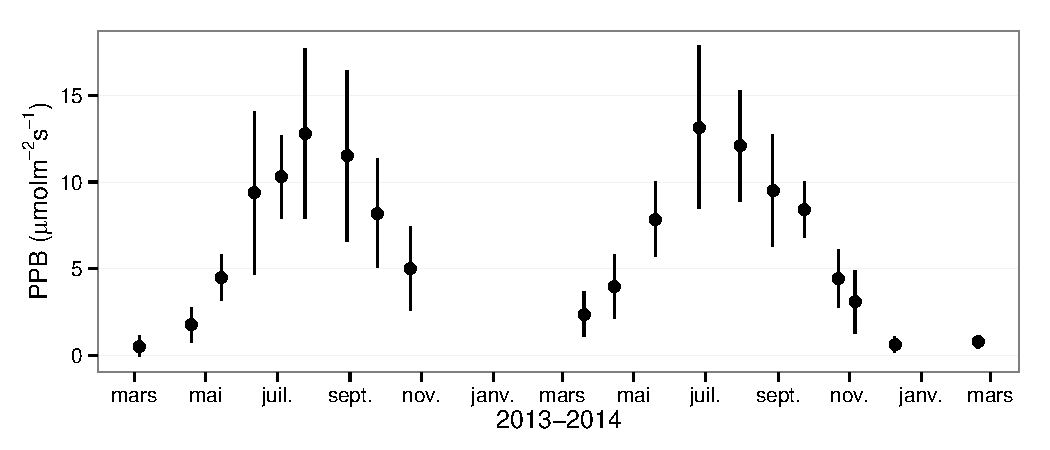
\includegraphics[width=\textwidth]{chap3/GPP_evolution_avg}
%\caption{Évolution du niveau de la production primaire brute, moyenne des 20 embases pendant la période de mesure (mars 2013 -- février 2015)}
%\label{fig:GPP_evolution_avg}
%\end{figure}

%\subsubsection{ER}

La RE en 2013 augmente pendant le printemps et une partie de l'été, elle atteint un maximum de \SI{99999(888)}{\uml} en juillet avant de diminuer.
En 2014 la RE atteint, comme la PPB, son maximum plus tôt, en juin à \SI{99999(888)}{\uml} avant de décroître jusqu'en hiver pour approcher des valeurs nulles.
La moyenne annuelle de RE en 2013 est de \SI{4.27(316)}{\uml}, ce qui est légèrement supérieure à celle de 2014 : \SI{3.63(256)}{\uml}(Figure~\ref{fig:ER_evolution_avg}).



%\begin{figure}
%\centering
%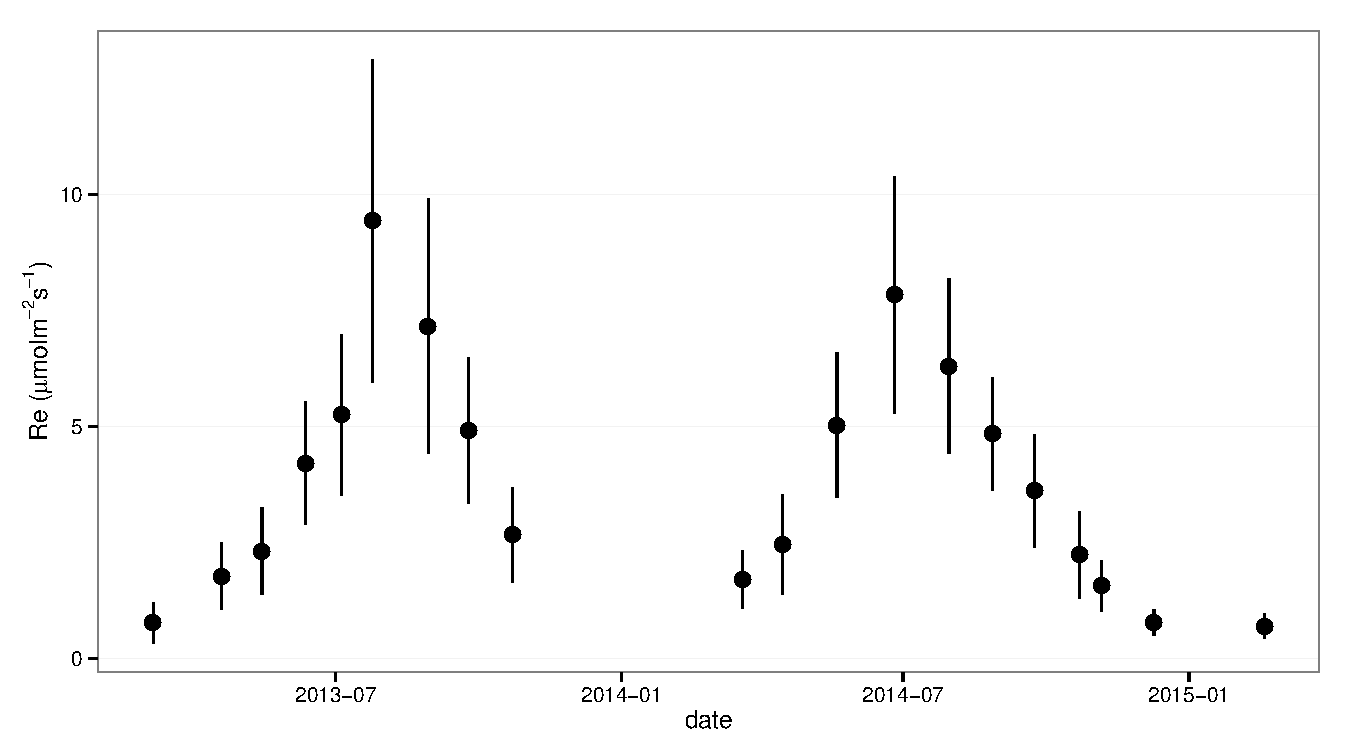
\includegraphics[width=\textwidth]{chap3/ER_evolution_avg}
%\caption{Évolution du niveau de la respiration de l'écosystème, moyenne des 20 embases pendant la période de mesure (mars 2013 -- février 2015)}
%\label{fig:ER_evolution_avg}
%\end{figure}

%\subsubsection{ENE}

Concernant l'ENE, en 2013 elle augmente jusqu'en juin avec un maximum à \SI{99999(888)}{\uml} avant de diminuer jusqu'à la fin de l'année.
Cependant, cette baisse est moins homogène que celle des deux flux précédents, avec notamment une augmentation de l'ENE entre juillet et août 2013.
Ceci étant, il faut également noter les valeurs importantes de la déviation standard particulièrement en juin et en août.
En 2014, l'ENE maximum est atteinte en juillet avec \SI{99999(888)}{\uml} avant qu'elle ne décroisse.
Cette baisse est cependant plus homogène qu'en 2013.
les moyennes de l'ENE en 2013 et 2014 sont très proche est sont respectivement de \SI{2.85(305)}{\uml} et \SI{2.93(277)}{\uml} (Figure~\ref{fig:NEE_evolution_avg}).

\subsubsection{Le \chh}

Le \chh comme le \coo montre une variabilité saisonnière importante, cependant les flux mesurés sont un ordre de grandeur en dessous de ceux mesurés pour le \coo.
À l'inverse de ce dernier, l'importance des flux de \chh mesurés en 2013 et 2014 est différente.
En 2013 les flux sont moins important qu'en 2014 avec des maximum de \SIlist{0.078;0.196}{\uml} respectivement.

%\begin{figure}
%\centering
%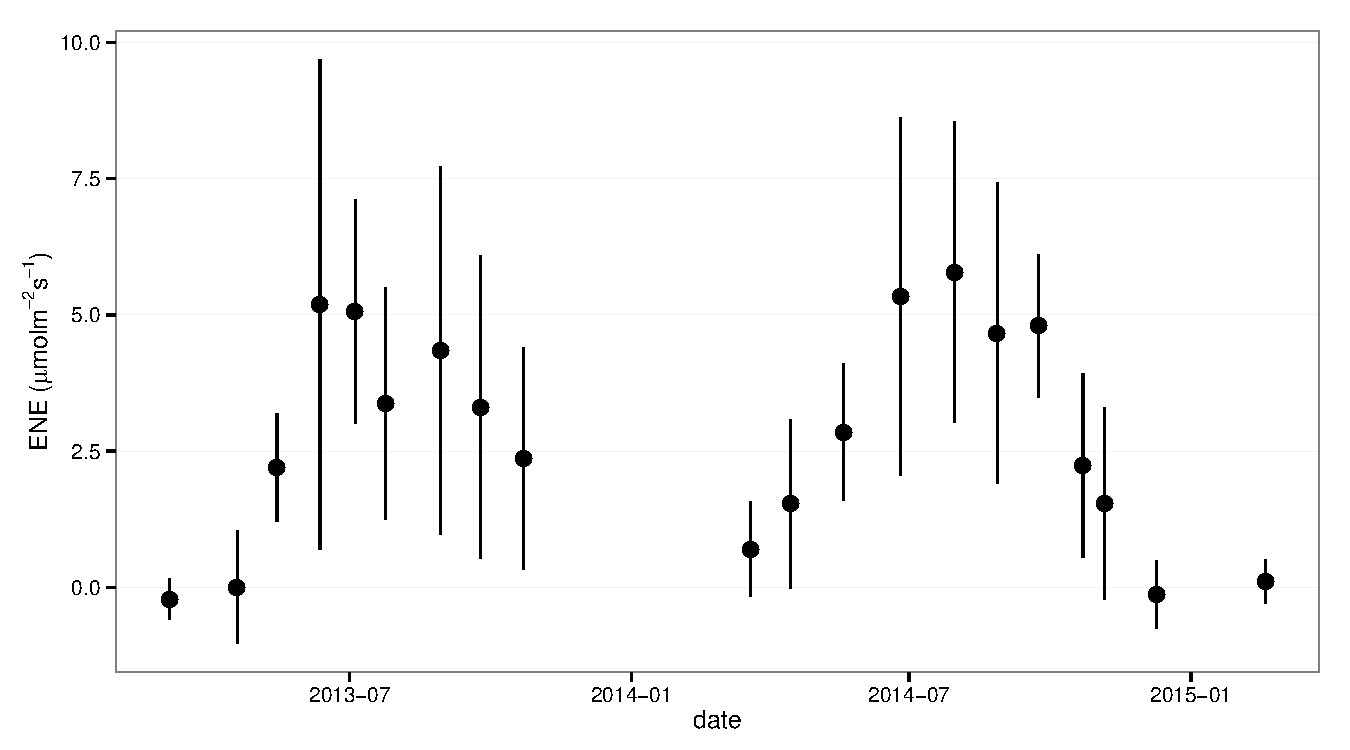
\includegraphics[width=\textwidth]{chap3/NEE_evolution_avg}
%\caption{Évolution du niveau de l'échange net de l'écosystème, moyenne des 20 embases pendant la période de mesure (mars 2013 -- février 2015)}
%\label{fig:NEE_evolution_avg}
%\end{figure}

\begin{figure}
\centering
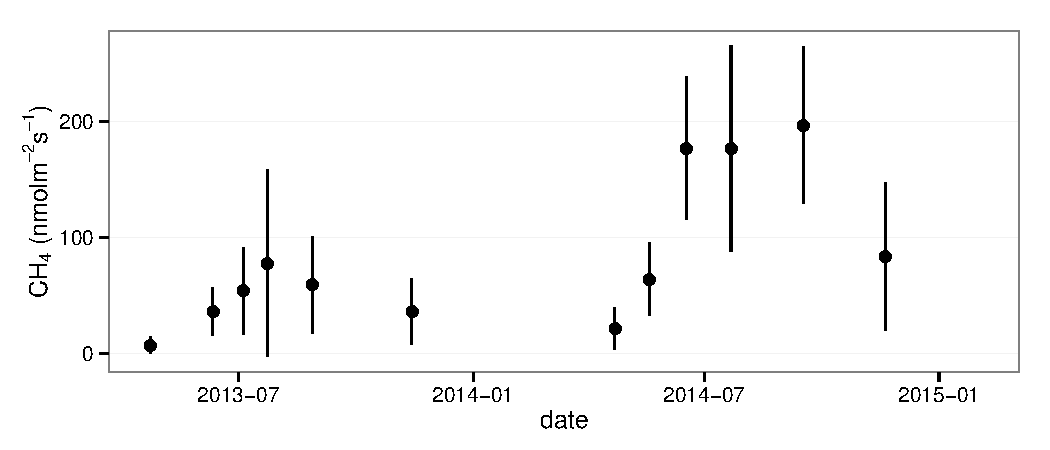
\includegraphics[width=\textwidth]{chap3/CH4_evolution_avg}
\caption{Évolution des flux de méthane moyen (N ?) pendant la période de mesure (mars 2013 -- février 2015)}
\label{fig:CH4_evolution_avg}
\end{figure}

\subsubsection{Le Carbone Organique Dissous (COD)}

\subsection{Le bilan de carbone de la tourbière de La Guette à l'échelle de l'écosystème}

%\subsubsection{Bilan de gaz annuel}

Afin de calculer le bilan à l'aide des équations XXXX, la température de l'air mesurée au niveau de la station météo à été utilisée.
Pour l'indice de végétation, le bilan a été calculé avec une interpolation linéaire entre les points.

\begin{figure}
\centering
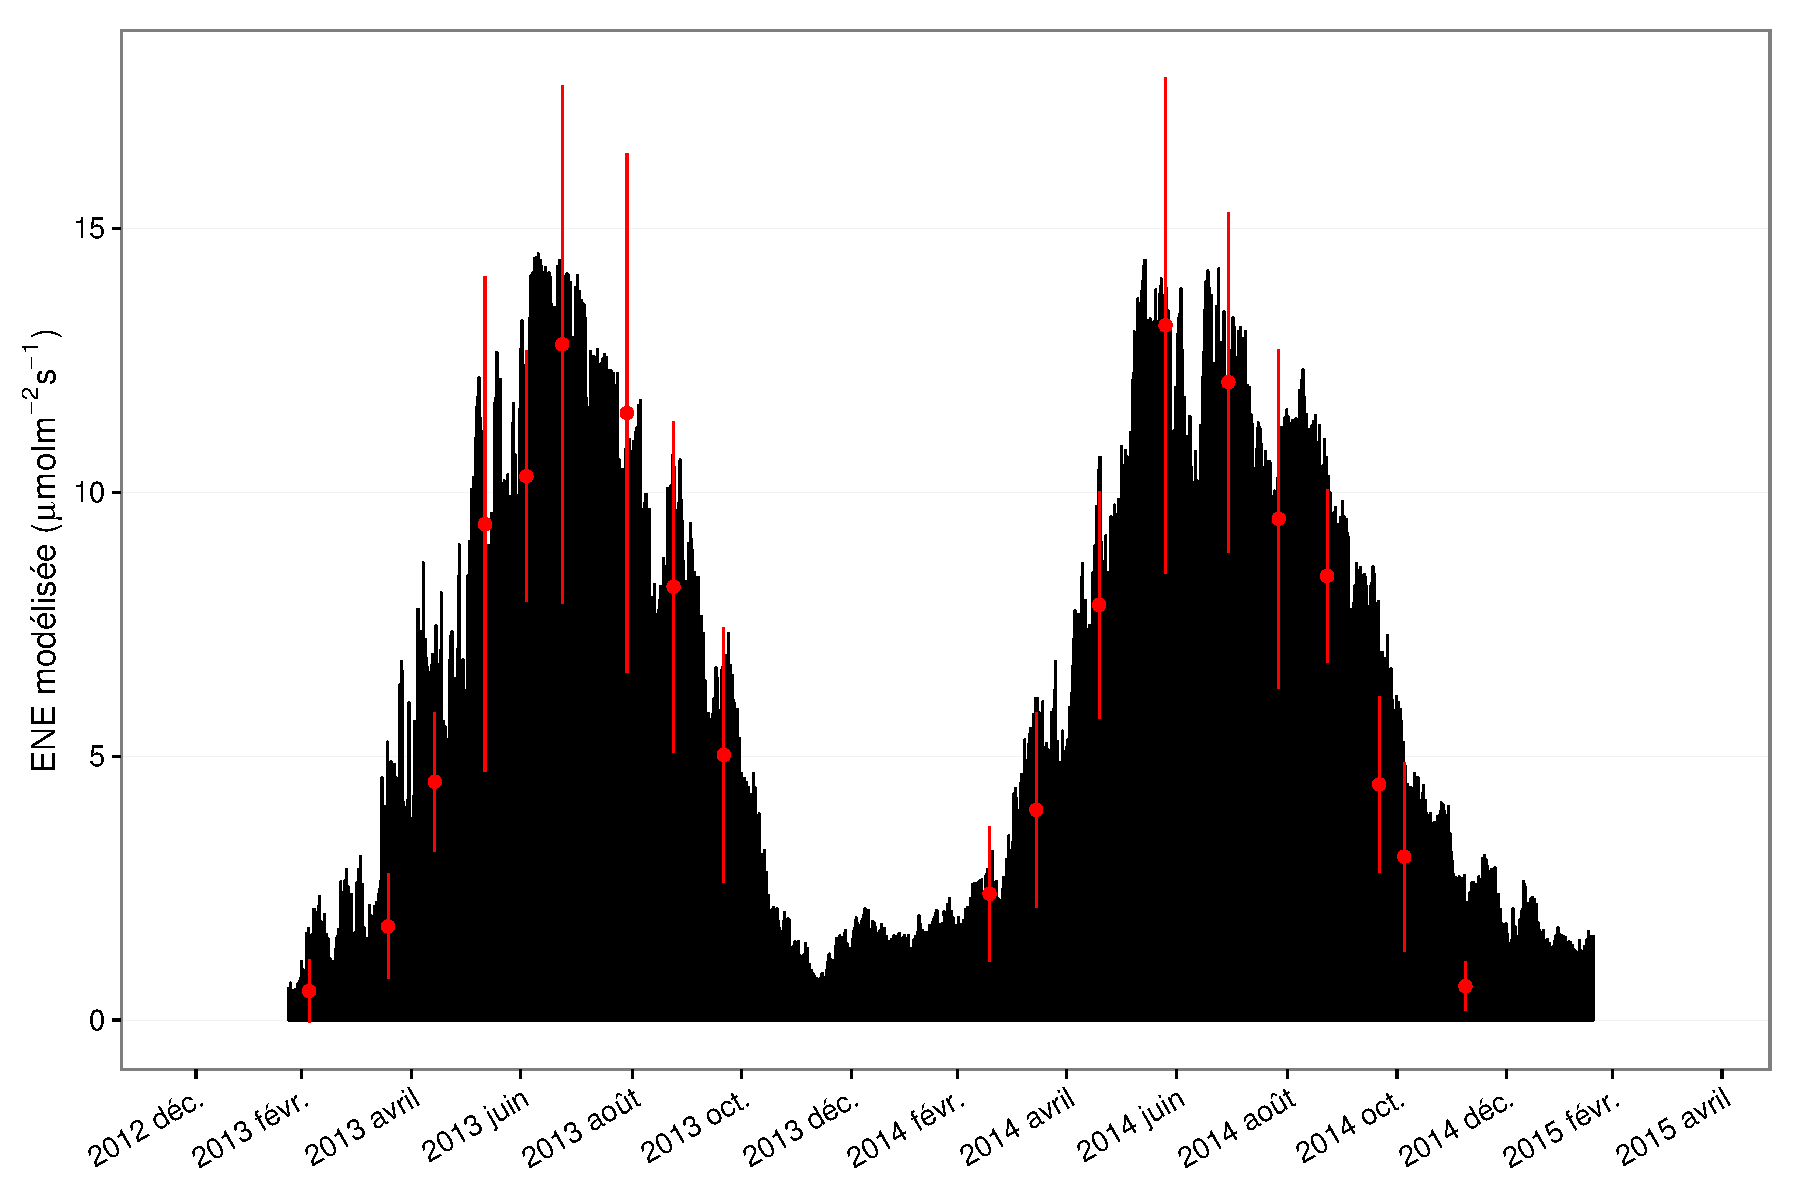
\includegraphics[width=\textwidth]{chap3/GPP_BdCitp_TairIVcov}
\caption{GPP interpolées à partir des équations~\ref{eq:juneTairIV} et \ref{eq:PPB_bubier})}
\label{fig:ENE_BdC_TairIVcov-T5}
\end{figure}

\begin{figure}
\centering
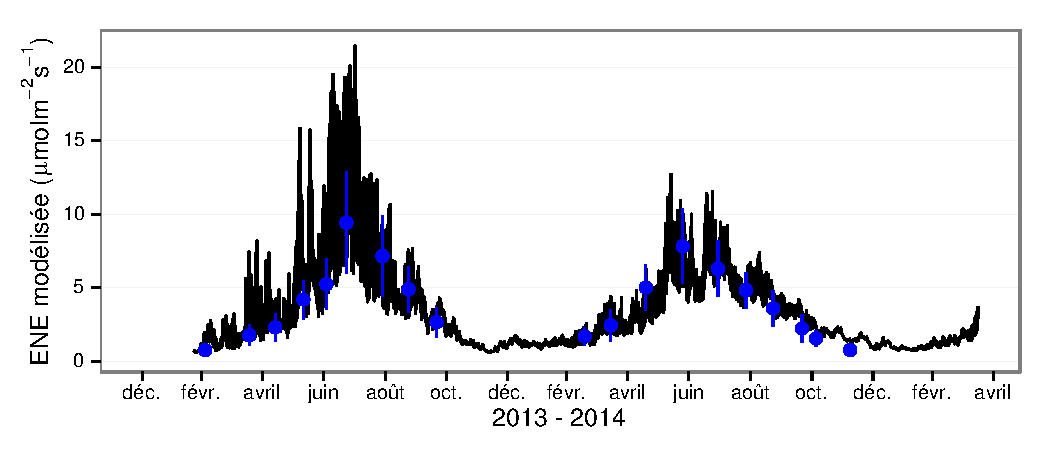
\includegraphics[width=\textwidth]{chap3/ER_BdCitp_T5}
\caption{RE interpolée à partir de l'équation~\ref{eq:RE_T5})}
\label{fig:RE_BdC_T5}
\end{figure}

\begin{figure}
\centering
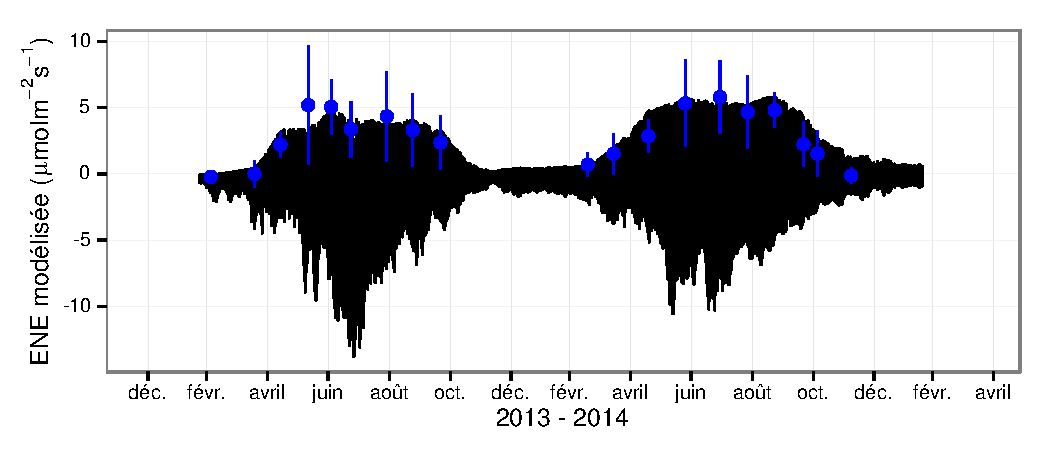
\includegraphics[width=\textwidth]{chap3/ENE_BdCitp_TairIVcov_T5}
\caption{ENE, PPB-RE, de la tourbière de La Guette}
\label{fig:PPB_BdC_TairIVcov}
\end{figure}

%\begin{figure}
%\centering
%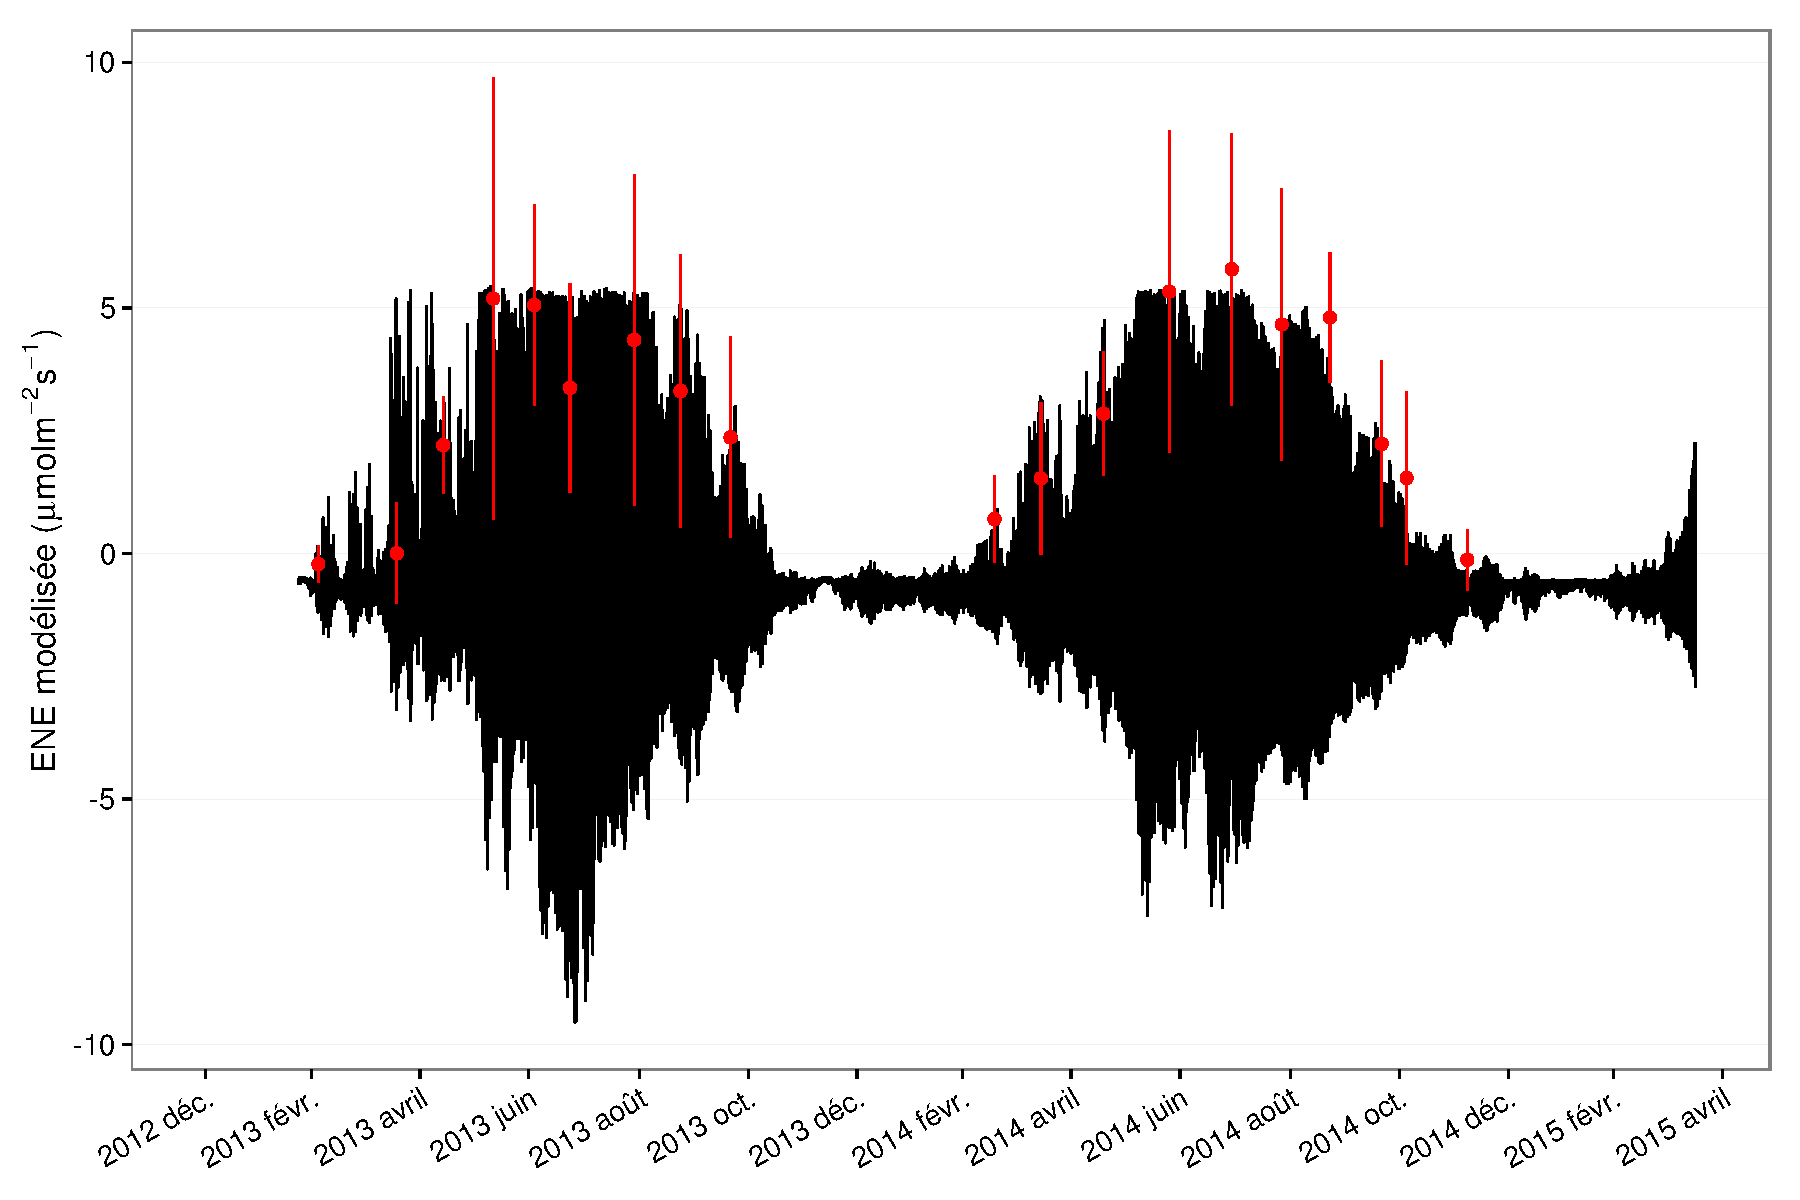
\includegraphics[width=\textwidth]{chap3/ENE_BdCitp_T5_T5}
%\caption{ENE modèles (2 variable explicative)}
%\label{fig:ENE_BdC_T5-T5_mod_mes}
%\end{figure}

%\begin{figure}
%\centering
%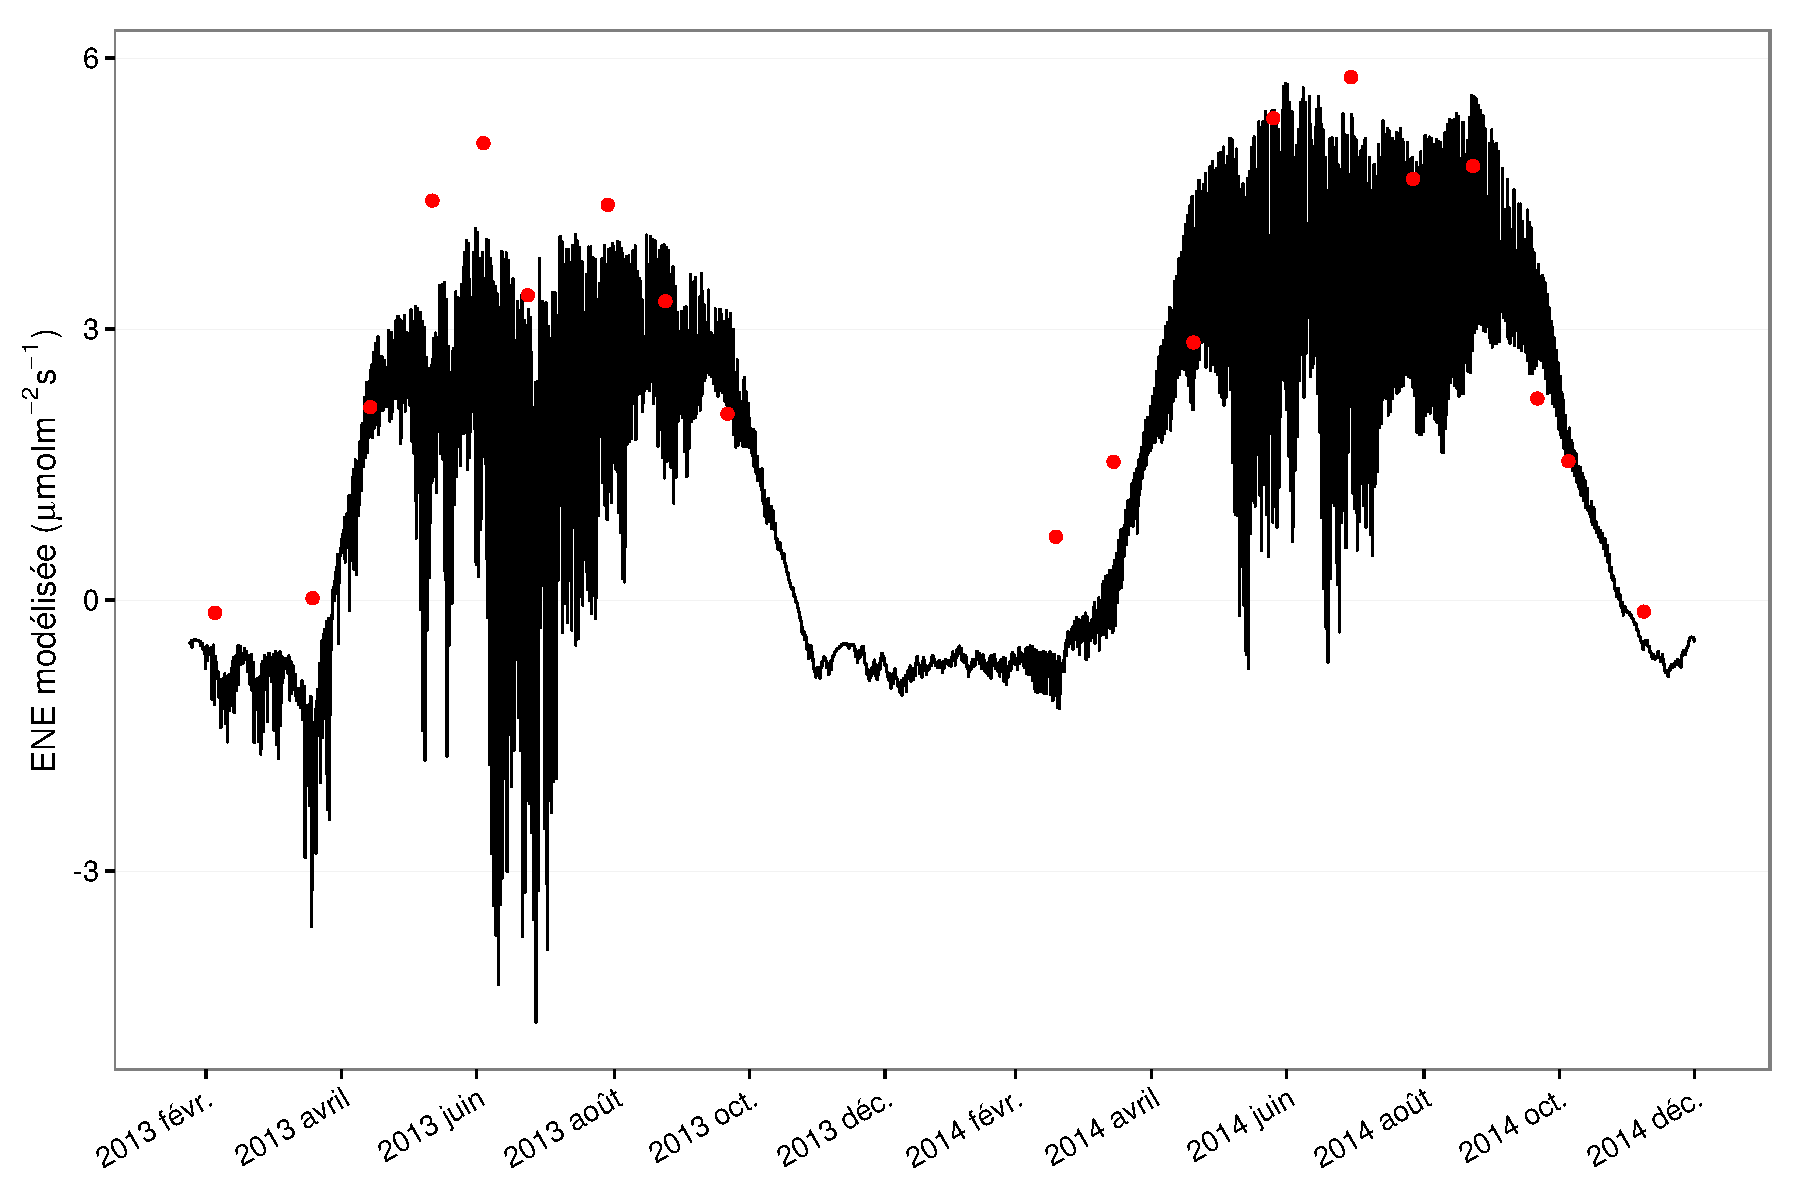
\includegraphics[width=\textwidth]{chap3/ENE_BdC_TairHH_mod_mes}
%\caption{ENE modèles (2 variable explicative)}
%\label{fig:ENE_BdC_TairHH_mod_mes}
%\end{figure}

%\begin{align}
%RE &= a \times exp(b\times T5)\\
%PPBsat &= a \times exp(-((Tair - b)/ c)^2)\\
%ENE &= PPB - RE\\
%ENE &= a \times exp(b\times T5) - a \times exp(-((Tair - b)/ c)^2)
%\end{align}


\subsection{Évaluation du bilan}

\subsubsection{sensibilité des paramètres}

L'analyse de sensibilité, consistant à faire varier chaque paramètre des modèles de $\pm$\SI{10}{\percent}, montre pour une équation exponentielle simple des valeurs attendues $\pm$\SI{10}{\percent} pour le paramètre a et \num{+29} à \SI{-22}{\percent} pour le b (Figure~\ref{table:mdl_sensitiv}).
Pour la PPB issue des équations~\ref{eq:juneTairIV} et \ref{eq:PPB_bubier} le paramètre i à très peu d'effet sur le bilan, \num{0} à \SI{-1}{\percent}.
Cependant l'effet sur le bilan augmente lorsque la végétation est prise en compte (équation~\ref{eq:juneTair} et \ref{eq:PPB_bubier}) : \num{-8} à \SI{-10}{\percent}.
À l'inverse, la sensibilité de l'ensemble des autres paramètres (a, b, c) diminue lorsque l'indice de végétation est pris en compte.
Le paramètre a est l'exception, passant de \num{-10} à \SI{-17}{\percent} pour une baisse de \SI{10}{\percent}.
Considérant le modèle de PPB prenant en compte la végétation, la sensibilité maximum des différents paramètres du bilan est proche de \SI{30}{\percent}, et similaire pour la PPB et la RE.

\begin{table}
\centering
\caption{Sensibilité relative (en \%) du bilan de \coo (ENE) en réponse à une variation de $\pm$\SI{10}{\percent} de chacun des paramètres des modèles.}
\label{table:mdl_sensitiv}
\begin{tabular}{llccc}\toprule
& & valeur & \SI{+10}{\percent} & \SI{-10}{\percent} \\ \midrule
RE & \multicolumn{4}{l}{équation~\ref{eq:RE_T5}} \\ 
& a & 0.34 & +10 & -10 \\
& b & 0.10 & +24 & -19 \\ [+1ex]
GPP & \multicolumn{4}{l}{équation~\ref{eq:juneTair} et \ref{eq:PPB_bubier}} \\
& a & 26.23 & +9 & -10 \\
& b & 53.68 & -36 & 44 \\
& c & 27.21 & +22 & -23 \\
& i & 1.84 & 0 & -1 \\ [+1ex]
GPP & \multicolumn{4}{l}{équation~\ref{eq:juneTairIV} et \ref{eq:PPB_bubier}} \\ 
& a & 33.66 & -1 & -17 \\
& b & 42.45 & -27 & 8 \\
& c & 25.77 & -1 & -18 \\
& i & 0.33 & -8 & -10 \\
\bottomrule
\end{tabular}
\end{table}

\subsubsection{pseudo-validation et erreur}

\begin{figure}
\centering
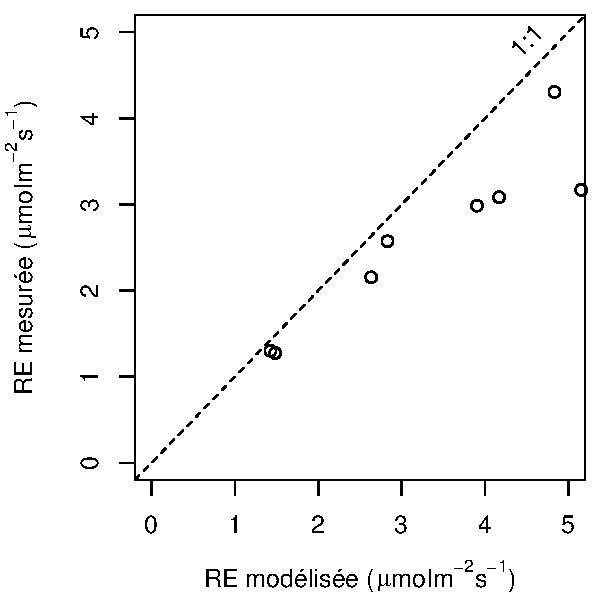
\includegraphics[width=.5\textwidth]{chap3/ER_T5_val}
\caption{Évaluation RE}
\label{fig:RE_T5_val}
\end{figure}
\begin{figure}
\centering
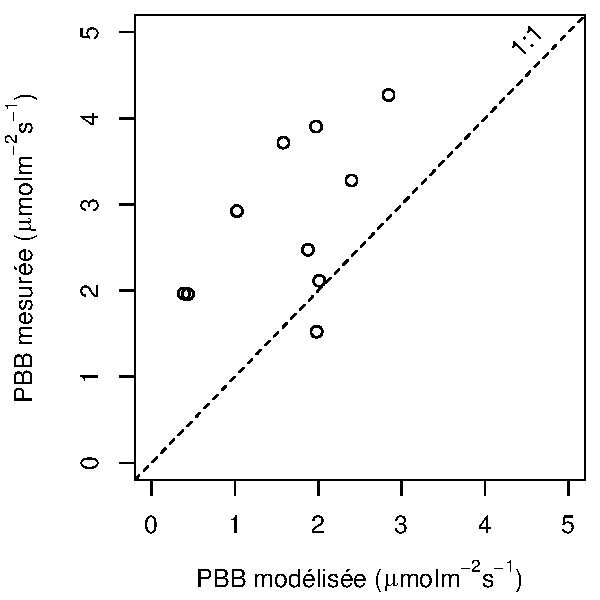
\includegraphics[width=.5\textwidth]{chap3/GPP_TairIVcov_val}
\caption{Évaluation GPP}
\label{fig:GPP_TairIVcov_val}
\end{figure}

\subsubsection{représentativité locale}


\section{Discussion}

\subsection{Représentativité du modèle à l'échelle de l'écosystème}

Valeur absolue des flux

Différence entre 2013 et 2014

apport d'un indice de végétation


\subsection{Représentativité locale du modèle}

\subsection{Sensibilité et limitations du bilan}


